\documentclass[10pt]{beamer}

%packages
\usepackage{babel}
\usepackage[utf8]{inputenc}
\usepackage{amsmath,tabu}
\usepackage{color}
\usepackage{tikz}
\usepackage{pgfplots}
\usepackage{colortbl}
\usetikzlibrary{calc,shadings}
\usetikzlibrary{positioning}
\usepackage{eurosym}
\usepackage{mathtools}

%definitions
\usepackage{algorithm,algorithmic}

%theme
\usetheme{Dresden}
\usecolortheme{rose}
\useoutertheme{tree}

%environments
\newenvironment{ExampleGer}{\begin{exampleblock}{Beispiel}}{\end{exampleblock}}

\newenvironment{customlegend}[1][]{%
	\begingroup
	% inits/clears the lists (which might be populated from previous
	% axes):
	\csname pgfplots@init@cleared@structures\endcsname
	\pgfplotsset{#1}%
}{%
	% draws the legend:
	\csname pgfplots@createlegend\endcsname
	\endgroup
}%

%definitions
\def\addlegendimage{\csname pgfplots@addlegendimage\endcsname}
% definition to insert numbers
\pgfkeys{/pgfplots/number in legend/.style={%
		/pgfplots/legend image code/.code={%
			\node at (0.295,-0.0225){#1};
		},%
	},
}

%general
\title{A Deep Neural Network Approach to Splice Site Prediction}
\author{Tilman Hinnerichs}
\institute{Knowledge Mining Lab -- KAUST}
\date{\today}

%presentation
\expandafter\def\expandafter\insertshorttitle\expandafter{%
	\insertshorttitle\hspace{7cm}%
	\insertframenumber\,/\,\inserttotalframenumber
}
\begin{document}
	
\begin{frame}
	\titlepage
\end{frame}

\begin{frame}{Outline}
	\setbeamertemplate{section in toc}[sections numbered]
	\tableofcontents
\end{frame}

\section{Problem Description}
\begin{frame}{Problem Description}
	\begin{figure}[ht]
		\centering
		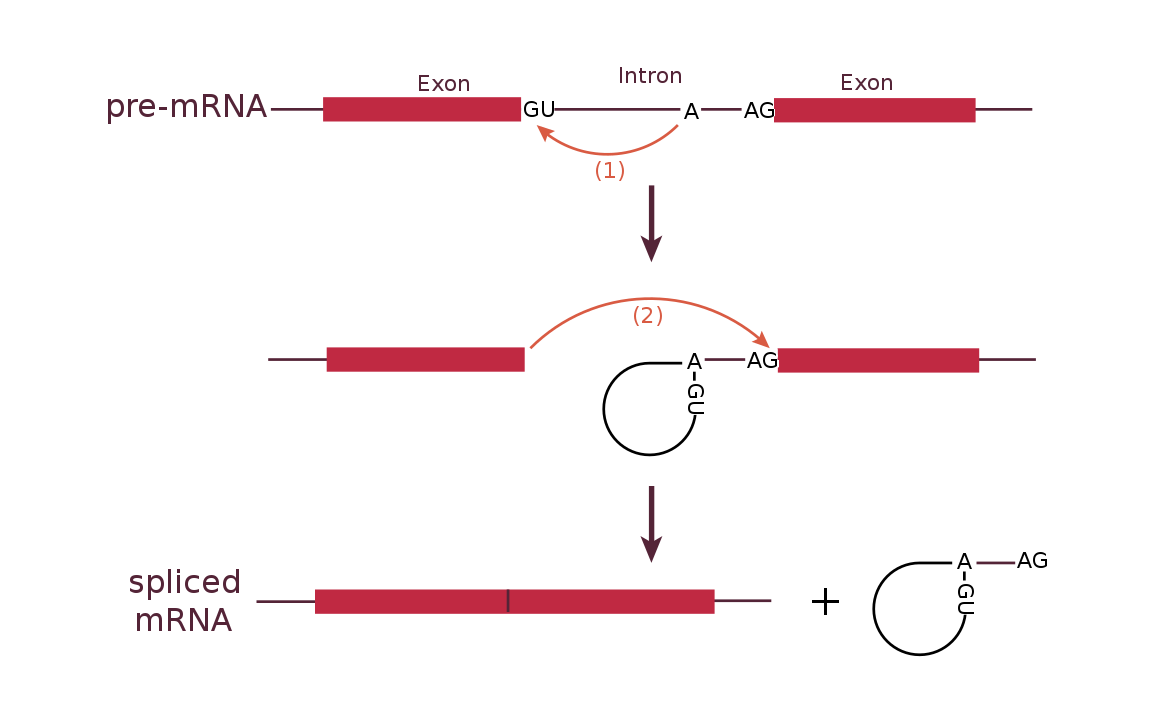
\includegraphics[width = 0.85\textwidth]{RNA_splicing_reaction.png}
		\caption{RNA splicing reaction}
	\end{figure}
\end{frame}

\begin{frame}{Problem Description}
	\large Splice side prediction on Arabidopsis thaliana genome
	\vspace{0.5cm}
	\pause
	\begin{itemize}
		\item Acceptor side:\\
			\dots CGTATCT\only{\colorbox{green}}<3->{AG}ATG\only{\colorbox{red}}<4->{AG}CA\dots
		\item Donor side:\\
			\dots ATGATTT\only{\colorbox{green}}<3->{GT}GCA\only{\colorbox{red}}<4->{GT}CA\dots
			
	\end{itemize}
\end{frame}

\section{Dataset description}
\begin{frame}{Dataset description}
	
	\large Example file, e.g., acceptor side
	\begin{align*}
		\begin{bmatrix}
		CT \dots \rotatebox{0}{\footnotesize $ 300 $ nt} \dots AG \dots \rotatebox{0}{\footnotesize $ 300 $ nt} \dots GC\\
		AG \dots \rotatebox{0}{\footnotesize $ 300 $ nt} \dots AG \dots \rotatebox{0}{\footnotesize $ 300 $ nt} \dots TT \\
		GA \dots \rotatebox{0}{\footnotesize $ 300 $ nt} \dots AG \dots \rotatebox{0}{\footnotesize $ 300 $ nt} \dots AA \\[0.2ex]
		\vdots\\
		\rotatebox{90}{\footnotesize$ ~100,000 $ records} \\[-1.3ex]
		\vdots \\[1.4ex]
		TT \dots \rotatebox{0}{\footnotesize $ 300 $ nt} \dots AG \dots \rotatebox{0}{\footnotesize $ 300 $ nt} \dots CC
		\end{bmatrix}
	\end{align*}
\end{frame}

\section{Classification Results}
\subsection{Baseline}
\begin{frame}{Classification results: Baseline}
	\large
	\begin{itemize}
		\item Build on label encoded data
		\item All models are validated by 10-fold cross validation
	\end{itemize}
	\begin{figure}
		\centering
		\begingroup
		\def\arraystretch{1.5}
		\begin{tabular}{|l|r|r|r|}
			\hline
			Approach & Samples & Acceptor acc. & Donor acc. \\
			\hline
			Naive Bayes & 40,000 & $79.32$ & $80.76$ \\
			Naive Bayes & 200,000 & $79.42$ & $81.12$ \\
			\hline
			SVM & 4,000 & 79.21 & 80.23\\
			\hline  
		\end{tabular}
		\endgroup
		\caption{Baseline results}
	\end{figure}	
\end{frame}

\subsection{Neural Networks}
\begin{frame}{Classification Results: NN -- binary classification}
	\begin{itemize}
		\item Models built on one-hot-encoded data
		\item Dense networks with dropout
	\end{itemize}
	\begin{figure}
		\centering
		\begingroup
		\def\arraystretch{1.2}
		\begin{tabular}{|l|r|r|r|r|}
			\hline
			Approach & Samples & Depth & Acceptor acc. & Donor acc. \\
			\hline
			NN & 40,000 & 1 & 62.24 & 63.15 \\
			\hline
			NN & 40,000 & 2 & 92.29 & 93.50 \\
			NN & 200,000 & 2 & 93.62 & 93.62 \\
			\hline
			DNN & 40,000 & 4 & 92.21 & 93.53 \\
			\hline
			DNN & 20,000 & 6 & 92.49 & 93.87 \\
			\hline
			DNN & 20,000 & 7 & 92.38 & 93.43 \\
			DNN & 200,000 & 7 & 93.34 & 93.34 \\
			\hline
			DNN & 40,000 & 8 & 92.50 & 93.82 \\
			DNN & 200,000 & 8 & 93.25 & 93.20 \\
			\hline
			DNN & 40,000 & 15 & 91.78 & 92.94 \\
			
			\hline  
		\end{tabular}
		\endgroup
		\caption{Binary classification results}
	\end{figure}
\end{frame}

\section{Next Steps}
\begin{frame}{Next Steps}
	\begin{itemize}
		\item Adapt convolution techniques from other papers with same goal
		\item Vary pre and post marker nt sequence length
		\item Use DiProDB[Friedel et al., NAR, 2009] for input
		\item Utilize electron io interaction potential (EIIP) for prediction
	\end{itemize}
\end{frame}


\begin{frame}{Sources}
	Images:
	\begin{itemize}
		\item https://en.wikipedia.org/
	\end{itemize}
\end{frame}


\end{document}